
\begin{frame}{The Twitter dialect}
\begin{scriptsize}
\begin{itemize}
\item An opinion lexicon is a lists of terms labelled by sentiment.
\item Lexicons are widely used resources for sentiment analysis
\item They are normally composed of positive and negative words such as \textcolor[rgb]{0.00,0.00,1.00}{\textbf{happy, wonderful}} and 
 \item The words used in Twitter include many abbreviations, acronyms, and misspelled words, e.g., \textbf{lol}, \textbf{omg}, \textbf{hahaha}, \textbf{\#hatemonday}.
\item This words are \textbf{not} covered by most popular lexicons.
\item The manual creation of a Twitter-oriented opinion lexicon is a \textbf{time-consuming} task.
\end{itemize}
\end{scriptsize}
\end{frame}



\begin{frame}{Automatic Lexicon Induction}
\begin{scriptsize}

\begin{itemize} 
 \item The automatic induction of an affective lexicon is normally done by exploiting \textbf{relations} between a \textbf{small seed lexicon} and \textbf{unknown words} from a \textbf{textual} resource.
\item  Two type of resources can be used: a lexical database such as \textbf{WordNet}, or a \textbf{corpus of documents}. 
\end{itemize}



\begin{figure}[h!]
	\centering
	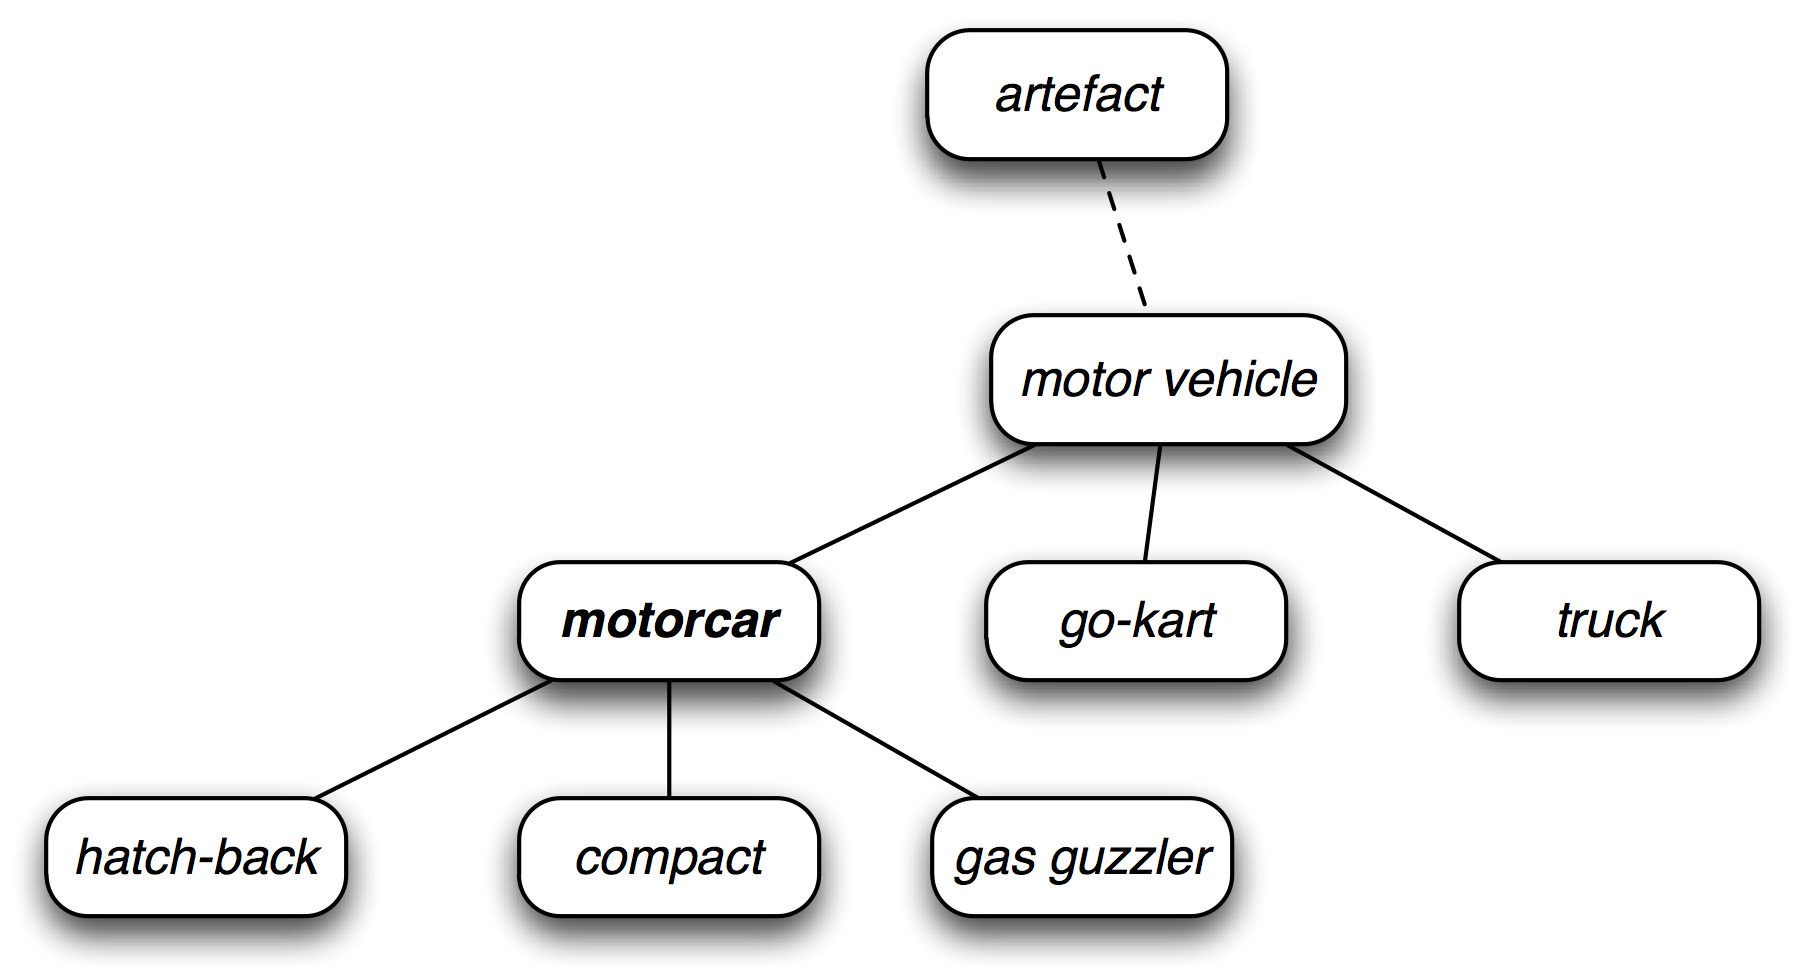
\includegraphics[scale=0.3]{pics/wordnet.png}
\end{figure}

\begin{figure}[h!]
	\centering
	
\includegraphics[scale=0.2]{pics/documents.jpg}
\end{figure}





\end{scriptsize}
\end{frame}



\begin{frame}{Lexicon expansion using WordNet}
\begin{scriptsize}

\begin{itemize} 
\item Methods based on WordNet expand the seed words using semantic relations such \textbf{synonyms} and \textbf{antonyms}, \cite{Liu2004,Kim2004}.
\item Hypothesis: synonyms have the \textbf{same} polarity and antonyms have the \textbf{opposite}.
\item In \cite{kamps2004} a \textbf{graph} was created using WordNet \textbf{adjectives} as vertices and the \textbf{synonym} relation as edges. 
\item Words are expanded by its \textbf{relative distance} from the two seed terms \textbf{good} and \textbf{bad}.
\item In \cite{Esuli2005, esuli2006} the authors take the \textbf{dictionary definitions} of the seed words to train a word-level classifier. 
\end{itemize}
\end{scriptsize}
\end{frame}






\begin{frame}{Corpus-based lexicon expansion}
\begin{scriptsize}
\begin{itemize}
\item As semantic databases cover a fixed vocabulary, they \textbf{cannot} capture domain dependent words. 
\item Corpus approaches exploit \textbf{statistical patterns} observed in document corpora. 
\item They can potentially be applied to any domain, and hence, are more suitable for \textbf{Twitter lexicon expansion}.  
\item Hartziva et. al \cite{Hatziva1997} used the  conjunction relations between adjectives.
\item Idea: adjectives connected with \textbf{and} tend to have the same polarity in the opposite way than adjectives connected with \textbf{but}.
\end{itemize}
\end{scriptsize}
\end{frame}

\begin{frame}{Corpus-based lexicon expansion (2)}
\begin{scriptsize}
\begin{itemize}
\item Turney et.al proposed the PMI \textbf{semantic orientation} (PMI-SO) metric \cite{turney2003measuring}.
\item Point-wise mutual information \textbf{PMI}: Information-theoretic association metric between discrete variables.
\item PMI-SO: calculated as the difference between the \textbf{PMI} of the word with a positive and a negative seed word.

\begin{equation}
 \operatorname{PMI}(term_{1}, term_{2})= \log_{2} \left ( \frac{Pr(term_{1} \wedge term_{2})}{Pr(term_{1})Pr(term_{2})} \right )
\end{equation}

\begin{equation}\label{eq:so}
 \operatorname{SO}(word) = \operatorname{PMI}(word, ``excellent") - \operatorname{PMI}(word, ``poor")
\end{equation}

\item The PMI values are estimated by the number of \textbf{hits} returned by a search engine.

\item The resulting PMI-SO score is a numerical value whose \textbf{sign} represents the word's polarity.

\item The magnitude of the value represents the \textbf{sentiment intensity}. 


\end{itemize}
\end{scriptsize}
\end{frame}




\begin{frame}{Twitter lexicon expansion using PMI-SO}
\begin{scriptsize}
\begin{itemize}
\item Previous Twitter lexicon induction models compute the PMI-SO between \textbf{corpus words} and tweet-level sentiment \textbf{labels}. 
\item The tweets are \textbf{automatically} labelled to polarity classes using \textbf{distant supervision} \cite{Mohammad2013, Zhou2014} or \textbf{self-training} \cite{avaya2013}. 
\item  Distant supervision methods rely on strong \textbf{sentiment signals} found in the message such as \textbf{emoticons} \cite{Mohammad2013, Zhou2014} or \textbf{hashtags}  \cite{Mohammad2013} to label the messages.
\item  Tweets where these signals are not observed are \textbf{discarded}. 
\end{itemize}

\begin{table}[htbp]
\centering
\begin{tabular}{|l|l|}
\hline
positive & negative \\ \hline
:) & :( \\ 
:-) & :-( \\ 
:D & =( \\ 
=) & :'(   \\ \hline
\end{tabular}
\end{table} 


\end{scriptsize}
\end{frame}


\begin{frame}{Lexicon Induction with Distributional Vectors}
\begin{scriptsize}
\begin{itemize}
\item \textbf{Distributional Hypothesis} \cite{harris1954}: words occurring in the same \textbf{contexts} tend to have similar meanings.
\item Or equivalently: ``a word is characterized by the \textbf{company} it keeps".
\item \textbf{Distributional representations}: words are represented by \textbf{high-dimensional vectors} based on the context's where they occur. 

\end{itemize}
\end{scriptsize}
\end{frame}

\begin{frame}{Lexicon Induction with Distributional Vectors}
\begin{scriptsize}
\begin{enumerate}
\item Calculate word distributional vectors from a corpus of unlabelled tweets.
\item Label some training words with a seed lexicon.
\item Train a classifier on the seed words.
\item Use the classifier to induce the sentiment of all words from the corpus.
\end{enumerate}
\end{scriptsize}
\end{frame}

\begin{frame}{Word-context Matrices}
\begin{scriptsize}
\begin{itemize}
\item Distributional vectors are built from word-context matrices $M$. 
\item Each cell $(i,j)$ is a co-occurrence based association value between a \textbf{target word} $w_i$ and a \textbf{context} $c_j$ calculated  from a corpus of documents.
\item Contexts are commonly defined as windows of words surrounding $w_i$.
\item The window length $k$ is a parameter ( between 1 and 8 words on both the left and the right sides of $w_i$).
\item If the Vocabulary of the target words and context words is the same, $M$ has dimensionality $|\mathcal{V}| \times |\mathcal{V}|$.
\item Whereas shorter windows are likely to capture \textbf{syntactic information} (e.g, POS), longer windows are more likely to capture topical similarity \cite{goldberg2016primer, JurafskyBook}.
\end{itemize}

\end{scriptsize}
\end{frame}



\begin{frame}{Distributional Vectors with context windows of size 1}


\begin{figure}[htb]
	\centering
	 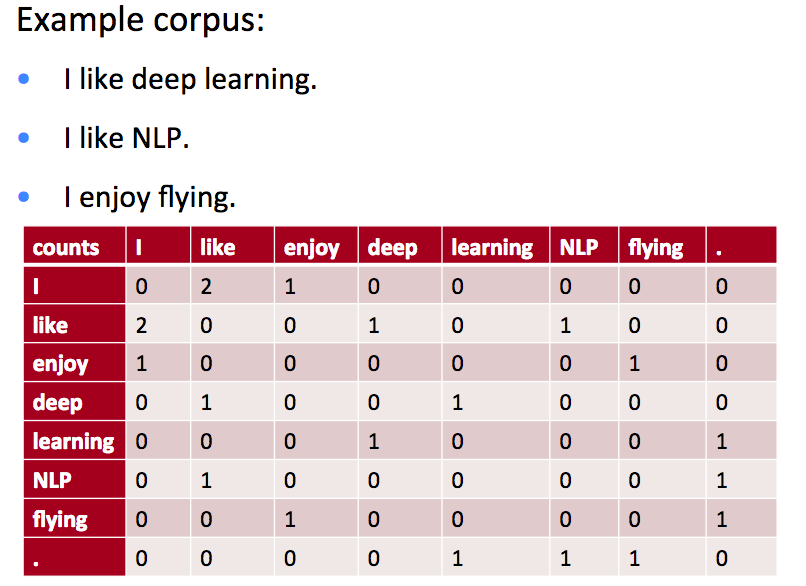
\includegraphics[scale=0.3]{pics/distributionalSocher.png}
\end{figure}


\footnotetext{Example taken from:    \url{http://cs224d.stanford.edu/lectures/CS224d-Lecture2.pdf}}
%\footnote{Source: \url{http://cs224d.stanford.edu/lectures/CS224d-Lecture2.pdf}}

\end{frame}



\begin{frame}{Word-context Matrices}
\begin{scriptsize}
The associations between words and contexts can be calculated using different approaches:
\begin{enumerate}
 \item Co-occurrence counts
\item Positive point-wise mutual information (PPMI)
\item The significance values of a paired t-test.  
\end{enumerate}

The most common of those according to \cite{JurafskyBook} is PPMI.

Distributional methods are also referred to as count-based methods.

\end{scriptsize}
\end{frame}



\begin{frame}{PPMI}
\begin{scriptsize}
\begin{itemize}
\item PPMI a filtered version of the traditional PMI measure in which negative values are set to zero:
\begin{equation}
 \operatorname{PPMI}(w, c)= \operatorname{max}(0,\operatorname{PMI}(w, c))
\end{equation}

\begin{equation}
 \operatorname{PPMI}(w,c)= \max \left (0, \log_{2} \left ( \frac{\operatorname{count}(w,c)\times |D|}{\operatorname{count}(w)\times \operatorname{count}(c)} \right )\right ). 
\end{equation}
\item  PMI calculates the log of the probability of word-context pairs occurring together over the probability of them being independent. 
\item Negative PMI values suggest that the pair co-occurs less often than chance. 
\item These estimates are unreliable unless the counts are calculated from very large corpora \cite{JurafskyBook}.
\item  PPMI corrects this problem by replacing negative values by zero. 
\end{itemize}
\end{scriptsize}
\end{frame}




\begin{frame}{Tweet-centroid Model}
\begin{scriptsize}
\begin{itemize}
\item Tweet Centroid Model \cite{Bravo-Marquez2015}: the \textbf{whole tweet} is treated as a word's context.
\item Tweets as \textbf{vectors} calculated from the \textbf{content}.
\item Word-level vectors are calculated based on the \textbf{centroids} of the \textbf{tweet-vectors} where a word occurs.
\item Rationale: words exhibiting a \textbf{certain polarity} are more likely used in contexts expressing the \textbf{same polarity} than in contexts exhibiting a \textbf{different one}. 
\end{itemize}
\end{scriptsize}
\end{frame}



\begin{frame}{Tweet-centroid Model (2)}


\begin{figure}[htb]
	\centering
	 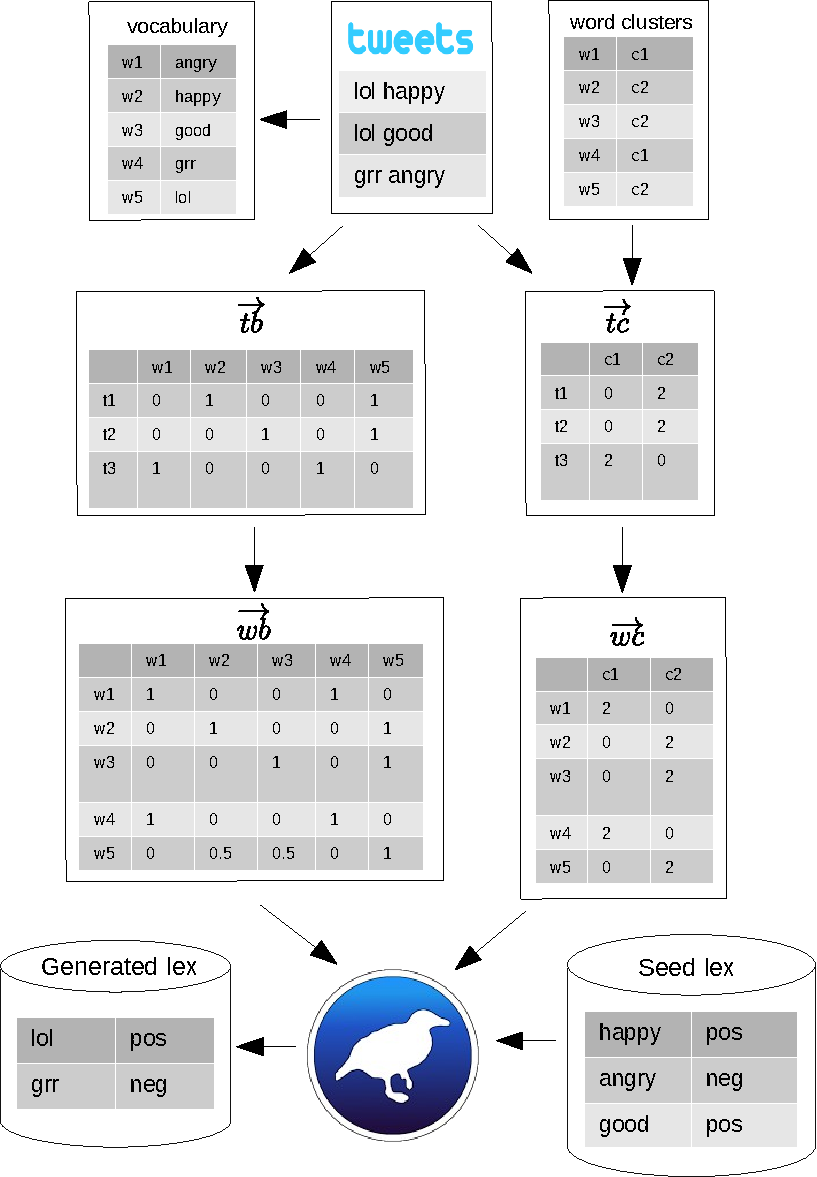
\includegraphics[scale=0.4]{sigirmodel.pdf}
\end{figure}



\end{frame}


\begin{frame}{Tweet-centroid Model (3)}
\begin{scriptsize}
\begin{itemize}
\item When unigrams are used it corresponds to a word-context matrix with whole tweets as contexts and associations calculated using co-occurrence counts normalised by the numbers of contexts where the target word appears.
\item Considering that the average number of words in a tweet is around 14 \cite{guo2013linking}, using tweets as contexts is similar to using windows of 14 words. 
\item The tweet centroid model admits arbitrary representations of contexts such as Brown clusters or other features capable of capturing useful semantic information. 
\item Traditional word-context matrices lack this property.
\end{itemize}
\end{scriptsize}
\end{frame}

\begin{frame}{Distributed Vectors or Word embeddings}
\begin{scriptsize}
\begin{itemize}

\item Count-based distributional vectors increase in size with vocabulary i.e., can have a very high dimensionality.

\item Explicitly storing the co-occurrence matrix can be memory-intensive. 

\item Some classification models don't scale well to high-dimensional data.

\item  The neural network community prefers using \textbf{distributed representations}\footnote{Idea: The meaning of the word is ``distributed'' over a combination of dimensions.} or \textbf{word embeddings}.

\item  Word \textbf{embeddings} are low-dimensional continuous dense word vectors trained from document corpora using \textbf{neural networks}.

\item They have become a crucial component of Neural Network architectures for NLP.


\end{itemize}
\end{scriptsize}
\end{frame}






\begin{frame}{Distributed Vectors or Word embeddings (2)}
\begin{scriptsize}
\begin{itemize}


\item They usually rely on an auxiliary predictive task (e.g., predict the following word).

\item The dimensions are not directly interpretable i.e., represent latent features of  the  word,  ``hopefully capturing useful syntactic and semantic properties''\cite{turian2010word}.

\item Most popular models are skip-gram \cite{Mikolov2013}, continuos bag-of-words \cite{Mikolov2013}, and Glove \cite{penningtonSM14}.

\item Word embeddings have shown to be more powerful than distributional approaches in many NLP tasks~\cite{baroni2014don}.

\item In \cite{amir2015SemEval}, they were used as \textbf{features} in a regression model for determining the association between Twitter words and \textbf{positive sentiment}. 

\end{itemize}
\end{scriptsize}
\end{frame}




\begin{frame}{Detour: Brief Introduction to Neural Networks}
\begin{scriptsize}
\begin{itemize}
\item Very popular machine learning models formed by units called \textbf{neurons}.
\item A neuron is a computational unit that has scalar inputs and outputs. 
\item  Each input has an associated weight $w$.
 \item The neuron multiplies each input by its weight, and then sums them (other functions such as \textbf{max} are also possible). 
\item It applies an activation function $g$ (usually non-linear) to the result, and passes it to its output.
\item Multiple layers can be stacked.
\end{itemize}


\end{scriptsize}
\end{frame}


\begin{frame}{Activation Functions}

\begin{scriptsize}
\begin{itemize}
\item The nonlinear activation function $g$ has a crucial role in the network's ability to represent complex functions. 
\item Without the nonlinearity in g, the neural network can only represent linear transformations of the input.
\end{itemize}


\end{scriptsize}

\begin{figure}[htb]
	\centering
	 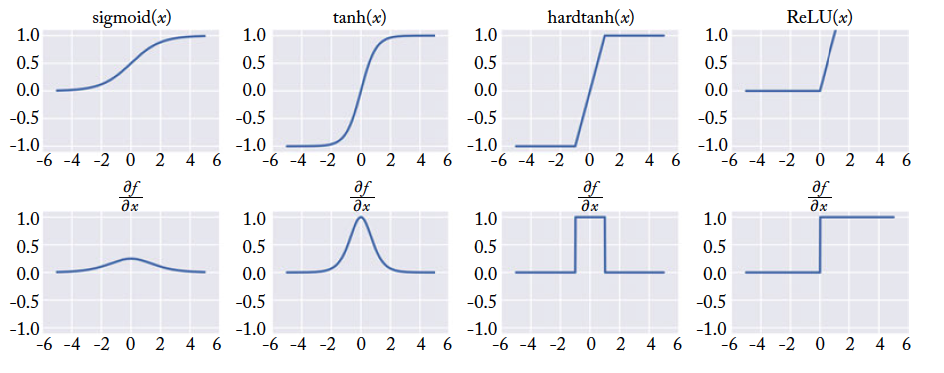
\includegraphics[scale=0.24]{pics/activations.png}
\end{figure}

\footnotetext{Source:\cite{goldberg2016primer}}

\end{frame}


\begin{frame}{Feedforward Network with two Layers}


\begin{figure}[htb]
	\centering
	 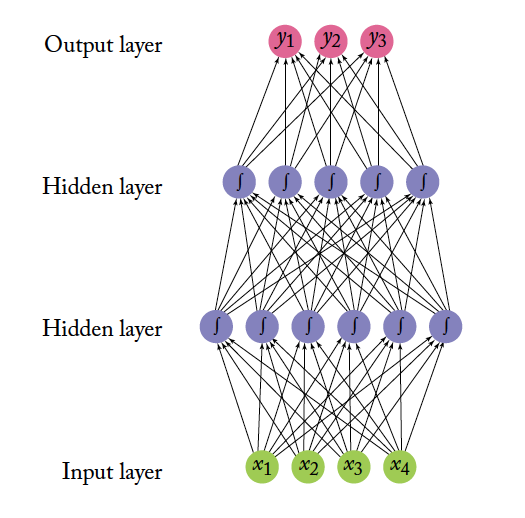
\includegraphics[scale=0.38]{pics/NN-example.png}
\end{figure}

\footnotetext{Source:\cite{goldberg2016primer}}

\end{frame}



\begin{frame}{Detour: Brief Introduction to Neural Networks}
\begin{scriptsize}
\begin{itemize}
\item The feedforward network from the picture is a stack of linear models separated by nonlinear functions.
\item The values of each row of neurons in the network can be thought of as a vector. 

\item The input layer is a 4-dimensional vector $(x)$, and the layer above it is a 6-dimensional vector $(h_1)$.
\item The fully connected layer can be thought of as a linear transformation from 4 dimensions to 6 dimensions. 
\item A fully connected layer implements a vector-matrix multiplication, $h=xW$.
\item The weight of the connection from the $i$-th neuron in the input row to the $j$-th neuron in the output row is $W_{[i,j]}$.
\item The values of $h$ are transformed by a nonlinear function $g$ that is applied to each value before being passed on as input to the next layer.

\end{itemize}


\end{scriptsize}
\end{frame}





\begin{frame}{Detour: Brief Introduction to Neural Networks}
\begin{scriptsize}
\begin{itemize}
\item The Multilayer Perceptron (MLP) from the figure can be written as the following mathematical function:
\begin{center}
\begin{equation}
\begin{split}
NN_{MLP2(x)} & =  y  \\
h^{1} &  = g^{1}(xW^{1}+b^{1}) \\
h^{2} &  = g^{2}(h^{1}W^{2}+b^{2}) \\
y &  = h^{2}W^{3}\\
y &  = (g^2(g^1(xW^{1}+b^{1})W^2+b^2))W^3.\\
\end{split}
\end{equation}
\end{center}
%NN_{MLP2(x)}  =  y \\
%h^{1} = g^{1}(xW^{1}+b{1}) \\

\end{itemize}


\end{scriptsize}
\end{frame}


\begin{frame}{Network Training}
\begin{scriptsize}
\begin{itemize}
\item  When training a neural network one defines a loss function $L(\hat{y}, y)$, stating the loss of predicting $\hat{y}$ when the true output is y.

\item The training objective is then to minimize the loss across the different training examples. 

\item Networks are trained using  gradient-based methods.

\item They work by repeatedly computing an estimate of the loss $L$ over the training set.

\item They compute gradients of the parameters with respect to the loss estimate, and moving the parameters in the opposite directions of the gradient. 

\item Different optimization methods differ in how the error estimate is computed, and how moving in the opposite direction of the gradient is defined.

\end{itemize}


\end{scriptsize}
\end{frame}




\begin{frame}{Online Stochastic Gradient Descent}


\begin{figure}[htb]
	\centering
	 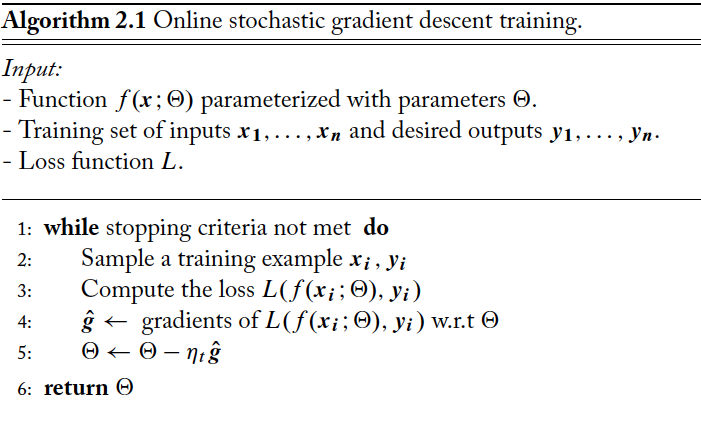
\includegraphics[scale=0.3]{pics/Online-SGD.png}
\end{figure}

\begin{scriptsize}
\begin{itemize}
\item The learning rate can either be fixed throughout the
training process, or decay as a function of the time step $t$.
\item  The error calculated in line 3 is based on a single training example, and is thus just a rough estimate of the corpus-wide loss $L$ that we are aiming to minimize. 
\item The noise in the loss computation may result in inaccurate gradients (single examples may provide noisy information).

\end{itemize}


\end{scriptsize}

\footnotetext{Source:\cite{goldberg2016primer}}

\end{frame}


\begin{frame}{Mini-batch Stochastic Gradient Descent}


\begin{scriptsize}
\begin{itemize}
\item A common way of reducing this noise is
to estimate the error and the gradients based on a sample of $m$ examples.
\item This gives rise to the minibatch SGD algorithm




\begin{figure}[htb]
	\centering
	 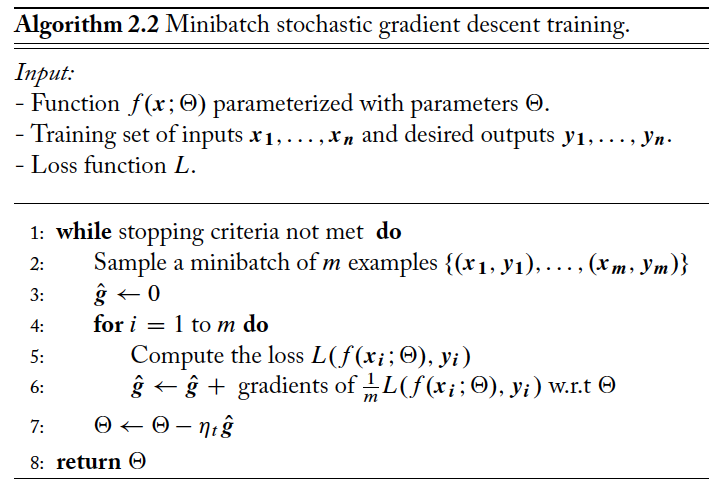
\includegraphics[scale=0.25]{pics/minibatch-SGD.png}
\end{figure}

\item Higher values of $m$ provide better estimates of the corpus-wide gradients, while smaller values allow more updates and in turn faster convergence.

\item For modest sizes of $m$ , some computing architectures (i.e., GPUs) allow an efficient parallel implementation of the computation in lines 3-6.

\end{itemize}
\end{scriptsize}

\footnotetext{Source:\cite{goldberg2016primer}}

\end{frame}



\begin{frame}{The Computation Graph Abstraction}
\begin{scriptsize}
\begin{itemize}
\item  One can compute the gradients of the various parameters of a network by hand and implement them in code.

\item This procedure is cumbersome and error prone.

\item For most purposes, it is preferable to use automatic tools for gradient computation [Bengio, 2012].

\item A computation graph is a representation of an arbitrary mathematical computation (e.g., a neural network) as a graph.

\item Consider for example a graph for the computation of $(a*b+1)*(a*b+2)$:

\begin{figure}[htb]
	\centering
	 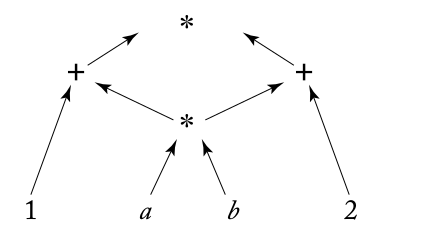
\includegraphics[scale=0.25]{pics/compGraph.png}
\end{figure}

\item The computation of $a*b$ is shared.

\item The graph structure defines the order of the computation in terms of the dependencies between the different components.

\end{itemize}
\end{scriptsize}
\end{frame}






\begin{frame}{The Computation Graph Abstraction}
\begin{scriptsize}
\begin{itemize}

\item  Te computation graph abstraction allows us to:


\begin{enumerate}
\begin{scriptsize}
 \item Easily construct arbitrary networks.
 \item Evaluate their predictions for given inputs (forward pass)
 
 \begin{figure}[htb]
	\centering
	 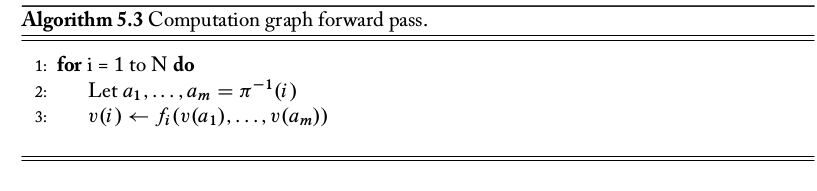
\includegraphics[scale=0.25]{pics/forwardPass.png}
\end{figure}

 
 
 \item Compute gradients for their parameters with respect to arbitrary scalar losses (backward pass or backpropagation).
 
 
  
 \begin{figure}[htb]
	\centering
	 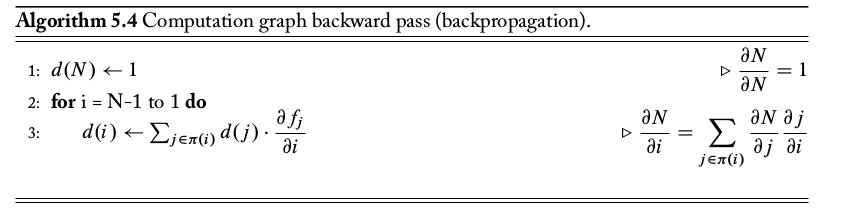
\includegraphics[scale=0.25]{pics/backwardPass.png}
\end{figure}
 
\end{scriptsize}
 \end{enumerate}
  
  
  
  
 \item The backpropagation algorithm (backward pass) is essentially following the chain-rule of differentiation\footnote{A comprehensive tutorial on the backpropagation algorithm over the computational graph abstraction: \url{https://colah.github.io/posts/2015-08-Backprop/}}.
 
 
 \item End of detour!
 
\end{itemize}
\end{scriptsize}
\end{frame}




\begin{frame}{Word2Vec}
\begin{scriptsize}
\begin{itemize}
\item Word2Vec is a software package that implements two neural network architectures for training word embeddings:  Continuos Bag of Words (CBOW) and Skip-gram.
\item It implements two  optimization models: Negative Sampling and Hierarchical Softmax.
\item These models are neural networks with one hidden layer that are trained to predict the contexts of words.
\end{itemize}
\end{scriptsize}
\end{frame}


% Good Word2Vec tutorial
%http://mccormickml.com/2016/04/19/word2vec-tutorial-the-skip-gram-model/

\begin{frame}{Skip-gram Model}
\begin{scriptsize}
\begin{itemize}
\item A neural network with one hidden layer is trained for predicting the words surrounding a center word, within a window  of size $k$ that is shifted along the input corpus. 
\item The center and surrounding $k$ words correspond to the input and output layers of the network.
\item Words are initially represented by 1-hot vectors: vectors of the size of the vocabulary ($|V|$) with zero values in all entries except for the corresponding word index that receives a value of 1. 
\item The output layer is formed by the concatenation of the $k$ 1-hot vectors of the surrounding words. 
\item The hidden layer has a dimensionality $d$, which determines the size of the embeddings (normally $d \ll |V|$).
\end{itemize}
\end{scriptsize}
  \begin{figure}[h]
        	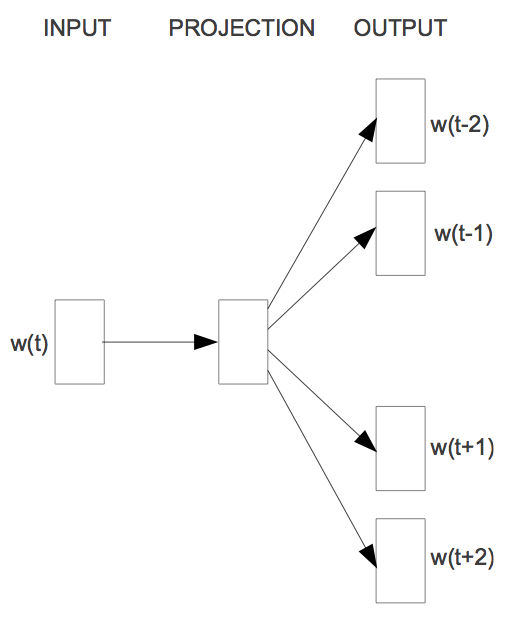
\includegraphics[scale = 0.33]{pics/skip-gram.png}
        \end{figure}

\end{frame}


\begin{frame}{Skip-gram Model}

  \begin{figure}[h]
        	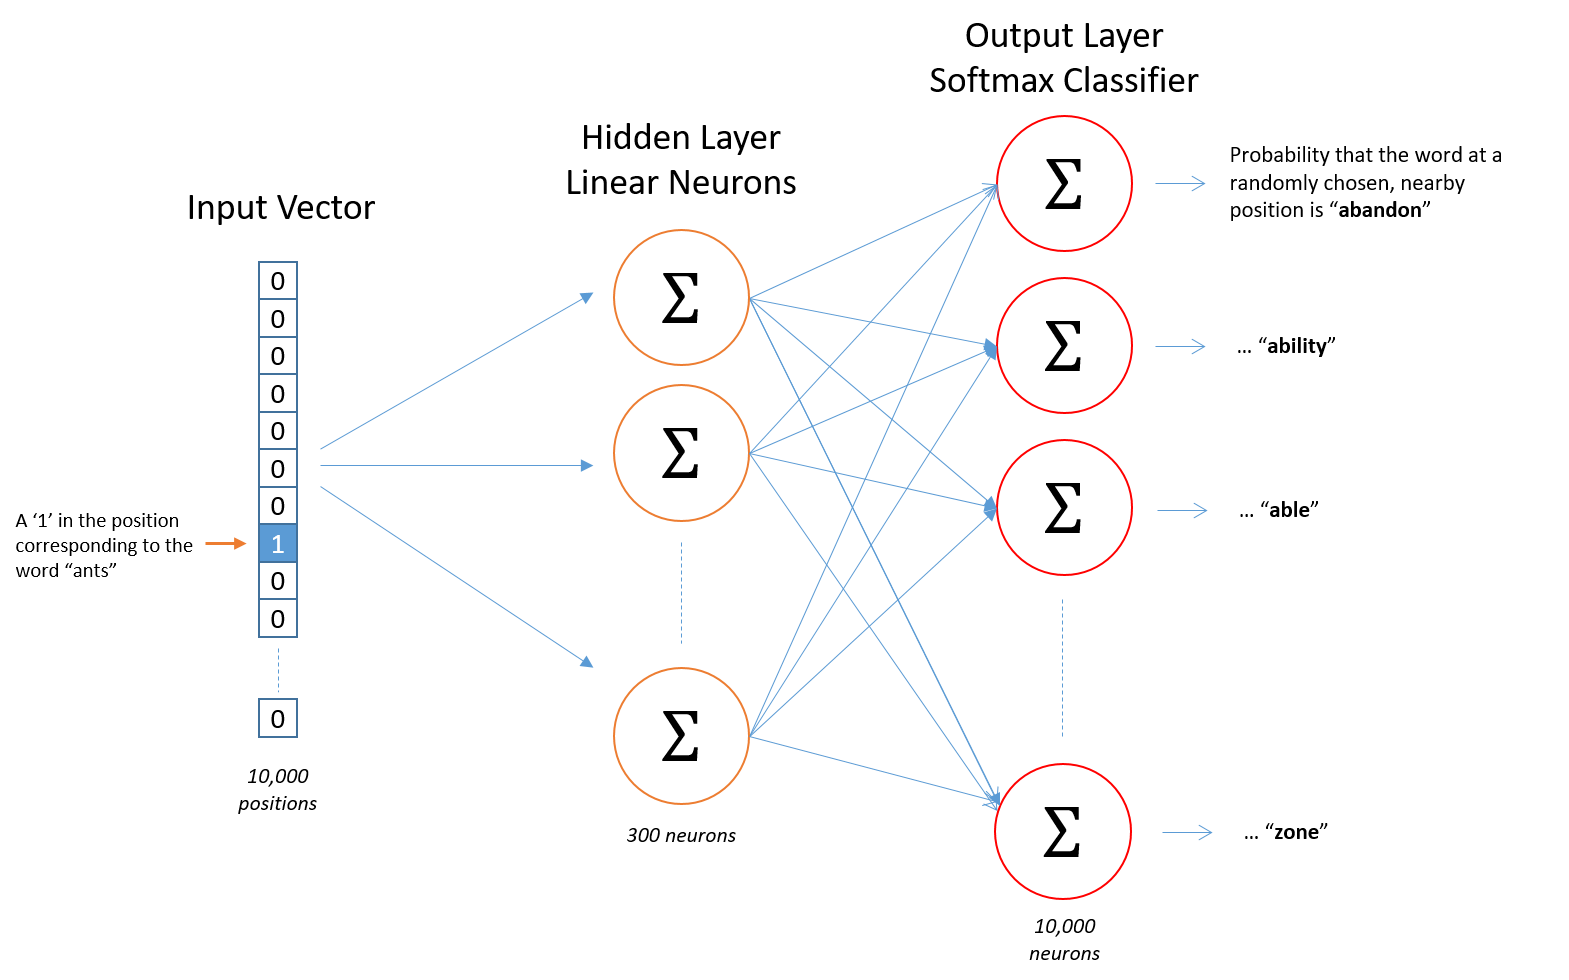
\includegraphics[scale = 0.4]{pics/skip_gram_net_arch.png}
        \end{figure}
\footnotetext{Picture taken from:    \url{http://mccormickml.com/2016/04/19/word2vec-tutorial-the-skip-gram-model/}}

\end{frame}


% we use hierarchical softmax where the vocabulary is represented as a Huffman binary tree. This follows previous observations that the frequency of words works well for obtaining classes in neural net language models [16]. Huffman trees assign short binary codes to frequent words, and this further reduces the number of output units that need to be evaluated


%If two different words have very similar “contexts” (that is, what words are likely to appear around them), then our model needs to output very similar results for these two words. And one way for the network to output similar context predictions for these two words is if the word vectors are similar. So, if two words have similar contexts, then our network is motivated to learn similar word vectors for these two words! Ta da!

%And what does it mean for two words to have similar contexts? I think you could expect that synonyms like “intelligent” and “smart” would have very similar contexts. Or that words that are related, like “engine” and “transmission”, would probably have similar contexts as well.

%This can also handle stemming for you – the network will likely learn similar word vectors for the words “ant” and “ants” because these should have similar contexts.

%https://arxiv.org/pdf/1402.3722.pdf

\begin{frame}{Parametrization of the Skip-gram model}
\begin{scriptsize}
\begin{itemize}
\item The conditional probability of the context word $c$ given the center word $w$ is modelled with a softmax ($C$ is the set of all context words):


\begin{displaymath}
p(c|w) = \frac{e^{\vec{c}\cdot \vec{w}}}{ \sum_{c'\in C} e^{\vec{c}'\cdot \vec{w}}}
\end{displaymath}



\item Model's parameters $\theta$: $\vec{c}$ and $\vec{w}$ (vector representations of contexts and words).
\item The optimization goal is to maximize the conditional likelihood of the contexts $c$:


\begin{equation}
\begin{split}
arg \max_{\vec{c}, \vec{w}} & \quad \sum_{(w,c) \in D}{\log p(c|w)} = \sum_{(w,c) \in D} ( \log e^{\vec{c}\cdot \vec{w}} - \log \sum_{c'\in C} e^{\vec{c}'\cdot \vec{w}}  )
\end{split}
\end{equation}


\item Assumption: maximising this function will result in good embeddings $\vec{w}$ i.e.,  similar words will have similar vectors.

\item The term $p(c|w)$ is computationally expensive because of the summation $\sum_{c'\in C} e^{\vec{c}'\cdot \vec{w}}$ over all the contexts $c'$

\item Fix: replace the softmax with a hierarchical softmax (the vocabulary is represented with a Huffman binary tree). 

\item Huffman trees assign short binary codes to frequent words, reducing the number of output units to be evaluated.

\end{itemize}
\end{scriptsize}
\end{frame}



%The distributional hypothesis states that words in similar contexts have similar meanings. The objective above clearly tries to increase the quantity  for good word-context pairs, and decrease it for bad ones.  Intuitively, this means that words that share many contexts will be similar to each other (notealso that contexts sharing many words will also be similar to each other). This is, however, very hand-wavy.

% https://arxiv.org/pdf/1402.3722.pdf  Skip-gram and Negative Sampling are not the same

\begin{frame}{Skip-gram with Negative Sampling}
\begin{scriptsize}
\begin{itemize}

\item Negative-sampling (NS) is presented as a more efficient model for calculating skip-gram embeddings. 
\item However, it optimises a different objective function \cite{goldberg2014word2vec}.

\item Let $D$ be the set of correct word-context pairs.

\item NS maximizes the probability that a word-context  pair a word-context pair $(w, c)$ came from the input corpus $D$ using a sigmoid function:

\begin{displaymath}
P(D = 1| w,c_i) = \frac{1}{1+e^{-\vec{w} \cdot \vec{c_{i}}}}
\end{displaymath}

\item Assumption: the contexts words $c_i$ are indepedent from each other:

\begin{displaymath}
P(D = 1| w,c_{1:k}) = \prod_{i=1}^{k}{P(D = 1| w,c_i)} = \prod_{i=1}^{k}{\frac{1}{1+e^{-\vec{w} \cdot \vec{c_{i}}}}} 
\end{displaymath}

\item This leads to the following target function (log-likelihood): 

\begin{equation}
\begin{split}
arg \max_{\vec{c}, \vec{w}} & \quad \log P(D = 1| w,c_{1:k}) = \sum_{i=1}^{k}{\log \frac{1}{1+e^{-\vec{w} \cdot \vec{c_{i}}}}}
\end{split}
\end{equation}





\end{itemize}
\end{scriptsize}
\end{frame}


\begin{frame}{Skip-gram with Negative Sampling (2)}
\begin{scriptsize}
\begin{itemize}


\item This objective has a trivial solution if we set $\vec{w}$,$\vec{c}$ such that $p(D=1|w,c)=1$ for every pair $(w,c)$ from $D$.
\item This is achieved by setting $\vec{w}=\vec{c}$  and $\vec{w} \cdot \vec{c} = K$ for all $\vec{w},\vec{c}$, where $K$ is a large number.
\item We need a mechanism that prevents all the vectors from having the same value, by disallowing some $(w, c)$ combinations. 
\item One way to do so, is to present the model with some $(w, c)$ pairs for which $p(D= 1|w, c)$ must be low, i.e.
pairs which are not in the data.  
\item This is achieved sampling negative samples from $\tilde{D}$. 





\end{itemize}
\end{scriptsize}
\end{frame}


\begin{frame}{Skip-gram with Negative Sampling (3)}
\begin{scriptsize}
\begin{itemize}

\item Sample $m$ words for each word-context pair  $(w,c) \in D$.
\item Add each sampled word $w_i$ together with the original context $c$ as a negative example to $\tilde{D}$.

%\item $\tilde{D}$ being $m$ times larger than $D$. 

%\item The number of negative samples $m$ is a parameter of the algorithm.

\item Final objective function:
\begin{equation}
\begin{split}
arg \max_{\vec{c}, \vec{w}} & \quad \sum_{(w,c) \in D}{\log P(D = 1| w,c_{1:k})} + \sum_{(w,c) \in \tilde{D}} \log P(D = 0| w,c_{1:k})
\end{split}
\end{equation}

\item The negative words are sampled from smoothed version of the corpus frequencies:
\begin{displaymath}
\frac{\#(w)^{0.75}}{\sum_{w'}\#(w')^{0.75}}
\end{displaymath}

\item This gives more relative weight to less frequent words.

\end{itemize}
\end{scriptsize}
\end{frame}






\begin{frame}{Continuos Bag of Words: CBOW}
\begin{scriptsize}
\begin{itemize}
\item  Similar to the skip-gram model but now the center word is predicted from the surrounding context.
 \begin{figure}[h]
    	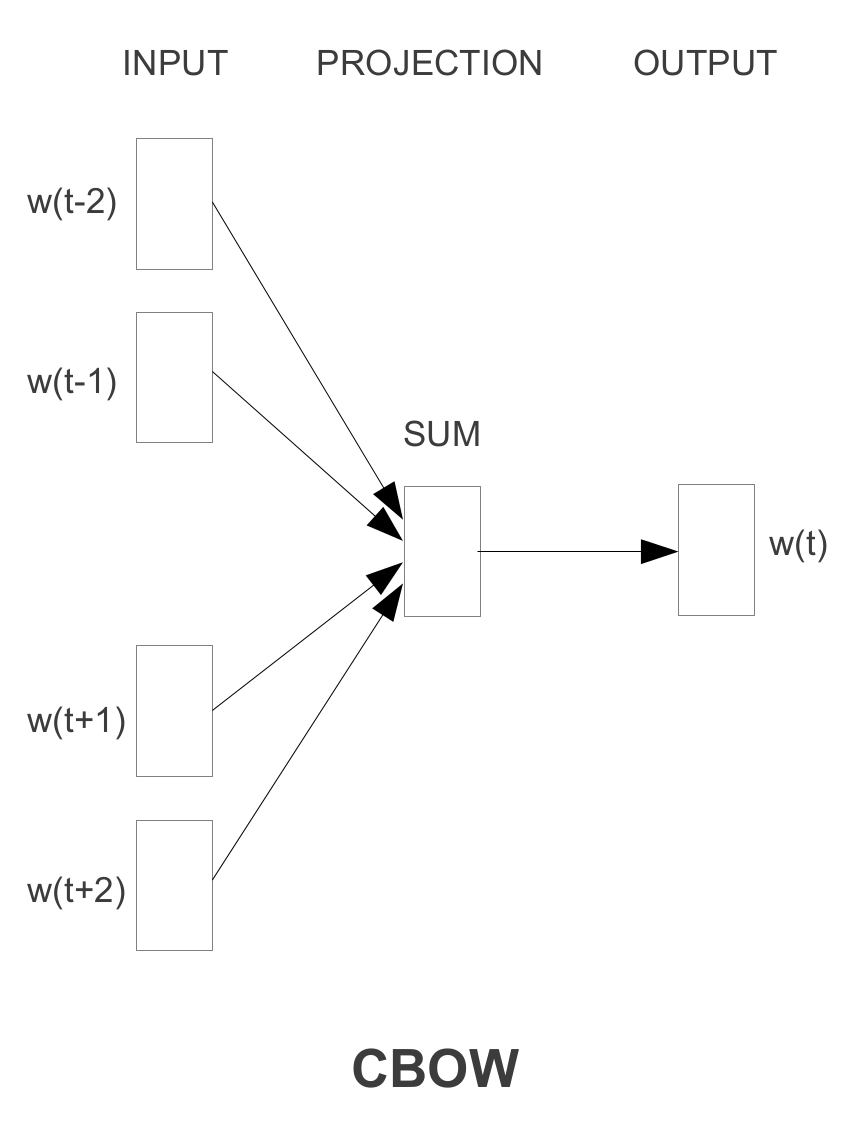
\includegraphics[scale = 0.55]{pics/CBOW.png}
    \end{figure}
       
        
\end{itemize}
\end{scriptsize}
\end{frame}



\begin{frame}{GloVe}
\begin{scriptsize}
\begin{itemize}
\item  GloVe (from global vectors) is another popular method for training word embeddings \cite{penningtonSM14}.

\item It constructs an explicit word-context
matrix, and trains the word and context vectors $\vec{w}$ and $\vec{c}$ attempting to satisfy:

\begin{equation}
w \cdot c + b_{[w]}+b_{[c]} = \log \#(w,c) \quad \forall (w,c) \in D
\end{equation}

\item where $b_{[w]}$ and $b_{[c]}$ are word-specific and context-specific trained biases.

        
\end{itemize}
\end{scriptsize}
\end{frame}



\begin{frame}{GloVe (2)}
\begin{scriptsize}
\begin{itemize}

\item In terms of matrix factorization, if we fix $b_{[w]}=\log \#(w)$ and $b_{[c]}=\log \#(c)$ we'll get an objective that is very similar to factorizing the word-context PMI matrix, shifted by $\log (|D|)$.
\item In GloVe the bias parameters are learned and not fixed, giving it another degree of freedom.

\item The optimization objective is weighted least-squares loss, assigning more weight to the correct reconstruction of frequent items.
       
\item When using the same word and context vocabularies, the model suggests representing each word as the sum of its corresponding word and context embedding vectors.   
        
\end{itemize}
\end{scriptsize}
\end{frame}


\begin{frame}{Word Analogies}
\begin{scriptsize}
\begin{itemize}
   
\item Word embeddings can capture certain semantic relationships, e.g. male-female, verb tense and country-capital relationships between words.

\item For example, the following relationship is found for word embeddings
trained using Word2Vec: $\vec{w}_{king} - \vec{w}_{man} + \vec{w}_{woman} \approx \vec{w}_{queen}$.

    
\end{itemize}

 \begin{figure}[h]
    	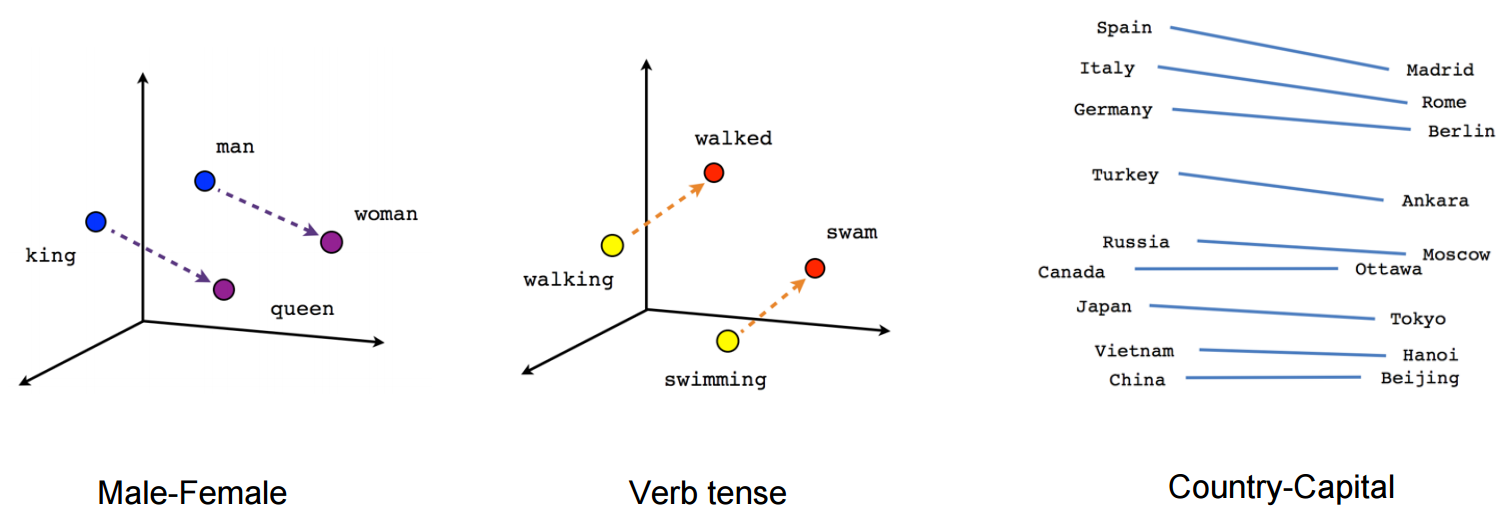
\includegraphics[scale = 0.2]{pics/linear-relationships.png}
    \end{figure}
\footnotemark{Source: \url{https://www.tensorflow.org/tutorials/word2vec}}

\end{scriptsize}
\end{frame}



\begin{frame}{Correspondence between Distributed and Distributional Models}
\begin{scriptsize}
\begin{itemize}
       
\item Both the distributional ``count-based'' methods and the distributed ``neural'' ones are based on the distributional hypothesis.

\item The both attempt to capture the similarity between words based on the similarity between the contexts in which they occur.      
       
\item Levy and Goldebrg showed in \cite{levy2014neural} that Skip-gram negative sampling (SGNS) is implicitly factorizing a word-context matrix, whose cells are the pointwise mutual information (PMI) of the respective word and context pairs, shifted by a global constant. 

%https://levyomer.files.wordpress.com/2014/09/neural-word-embeddings-as-implicit-matrix-factorization.pdf

\item This ties the neural methods and the traditional ``count-based'' suggesting that in a deep sense
the two algorithmic families are equivalent.
     
\end{itemize}
\end{scriptsize}
\end{frame}

\begin{frame}{Sentiment-Specific Phrase Embeddings}
%https://pdfs.semanticscholar.org/107f/b80ff801894b6191d0613af41aba91c134a4.pdf
\begin{scriptsize}
\begin{itemize}
\item Problem of word embeddings: antonyms can be used in similar contexts e.g., my car is nice vs my car is ugly.

\item In \cite{TangCol14}  \textbf{sentiment-specific} word embeddings are proposed  by combining the skip-gram model with emoticon-annotated tweets :) :( .

\item These embeddings are used for \textbf{training} a word-level polarity classifier.

\item The model integrates sentiment information into the continuous representation of phrases by developing a tailored neural architecture.

\item Input: $\{w_i,s_j,pol_j\}$, where $w_i$ is a phrase (or word), $s_j$ the sentence, and $pol_j$ the sentece's polarity.

\end{itemize}
\end{scriptsize}
\end{frame}


\begin{frame}{Sentiment-Specific Phrase Embeddings (2)}
%https://pdfs.semanticscholar.org/107f/b80ff801894b6191d0613af41aba91c134a4.pdf
\begin{scriptsize}
\begin{itemize}

\item The training objective uses the embedding of $w_i$ to predict its context words (in the same way as the skip-gram model), and uses the sentence representation $se_j$ to predict $pol_j$.


\item Sentences ($se_j$) are represented by averaging the word vectors of their words.

\item The  objective of the sentiment part is to maximize the average of log sentiment probability: 
\begin{displaymath}
f_{sentiment}= \frac{1}{S}\sum_{j=1}^{S}\log p(pol_j|se_j)
\end{displaymath}

\item The final training objective is to maximize the linear combination of the skip-gram and sentiment objectives: 
\begin{displaymath}
f = \alpha f_{skipgram} + (1- \alpha)f_{sentiment}
\end{displaymath}

\end{itemize}
\end{scriptsize}
\end{frame}



\begin{frame}{Sentiment-Specific Phrase Embeddings}
%https://pdfs.semanticscholar.org/107f/b80ff801894b6191d0613af41aba91c134a4.pdf


  \begin{figure}[h]
        	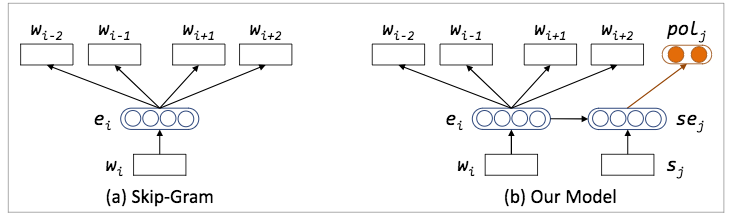
\includegraphics[scale = 0.4]{pics/SSPE.png}
        \end{figure}

  \begin{figure}[h]
        	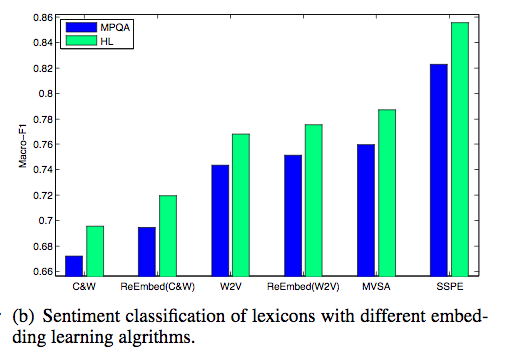
\includegraphics[scale = 0.3]{pics/SSPERes.png}
        \end{figure}


\end{frame}






\begin{frame}{Multi-Label Classification of Emotions with TCM}
\begin{scriptsize}

\begin{figure}[htbp]
\begin{center}
\scalebox{0.7}{
\begin{tabular}{cccc}
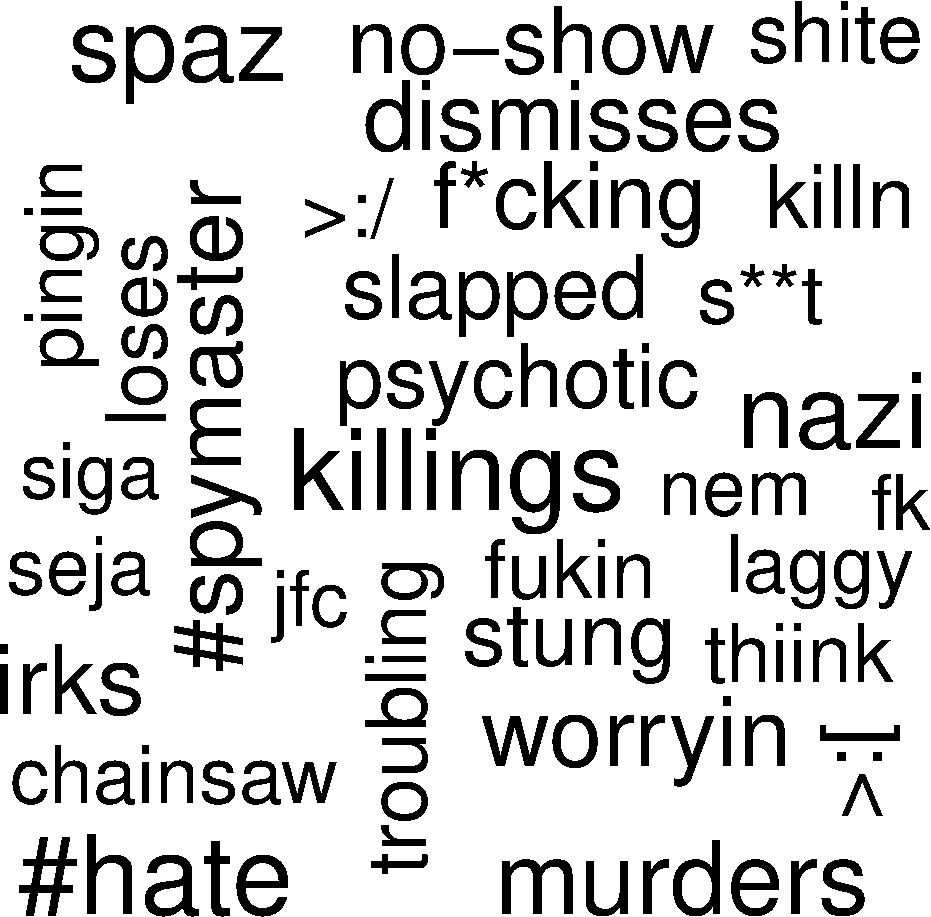
\includegraphics[scale=0.2]{pics/anger.pdf} & 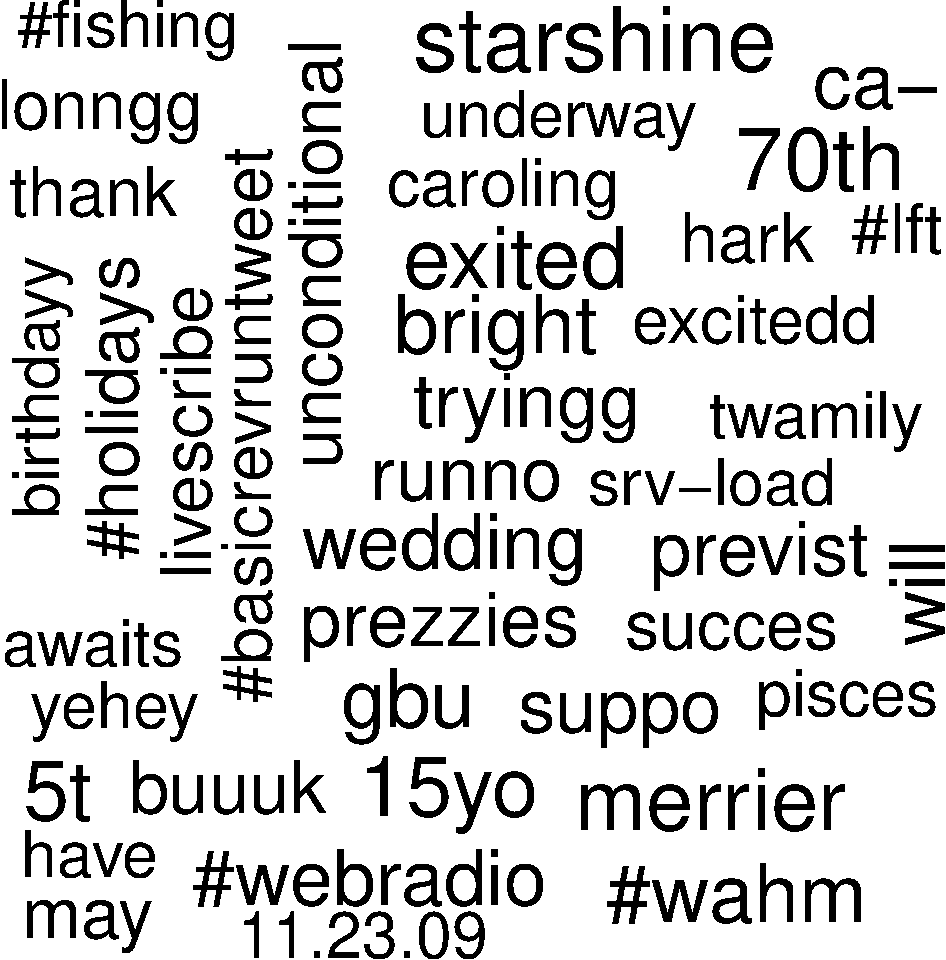
\includegraphics[scale=0.2]{pics/ant.pdf} & 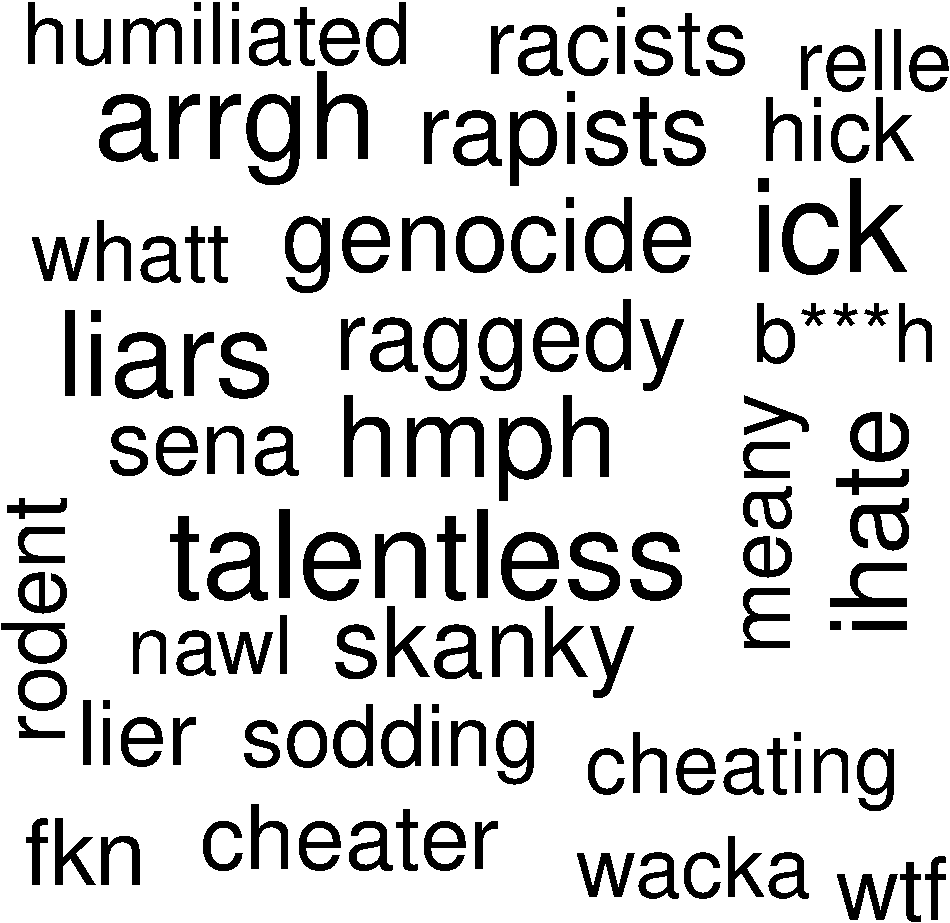
\includegraphics[scale=0.2]{pics/disg.pdf} & 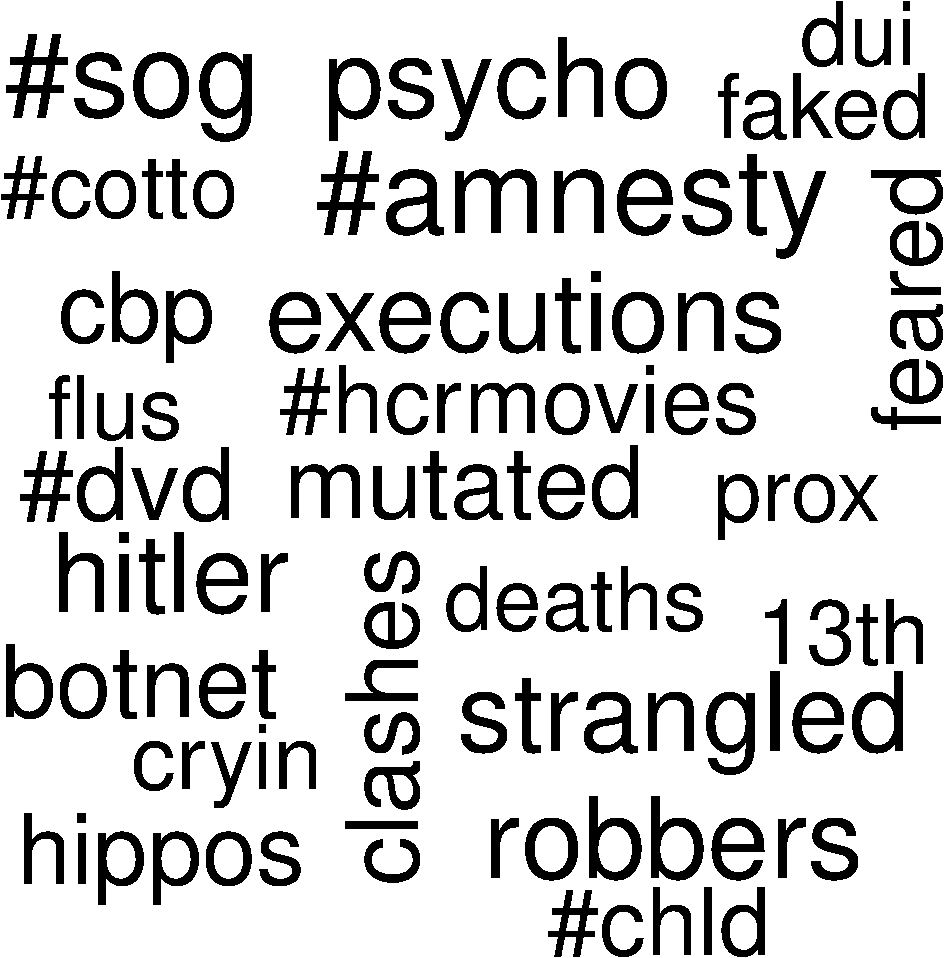
\includegraphics[scale=0.2]{pics/fear.pdf} \\
anger & anticipation & disgust & fear\\[1mm] 
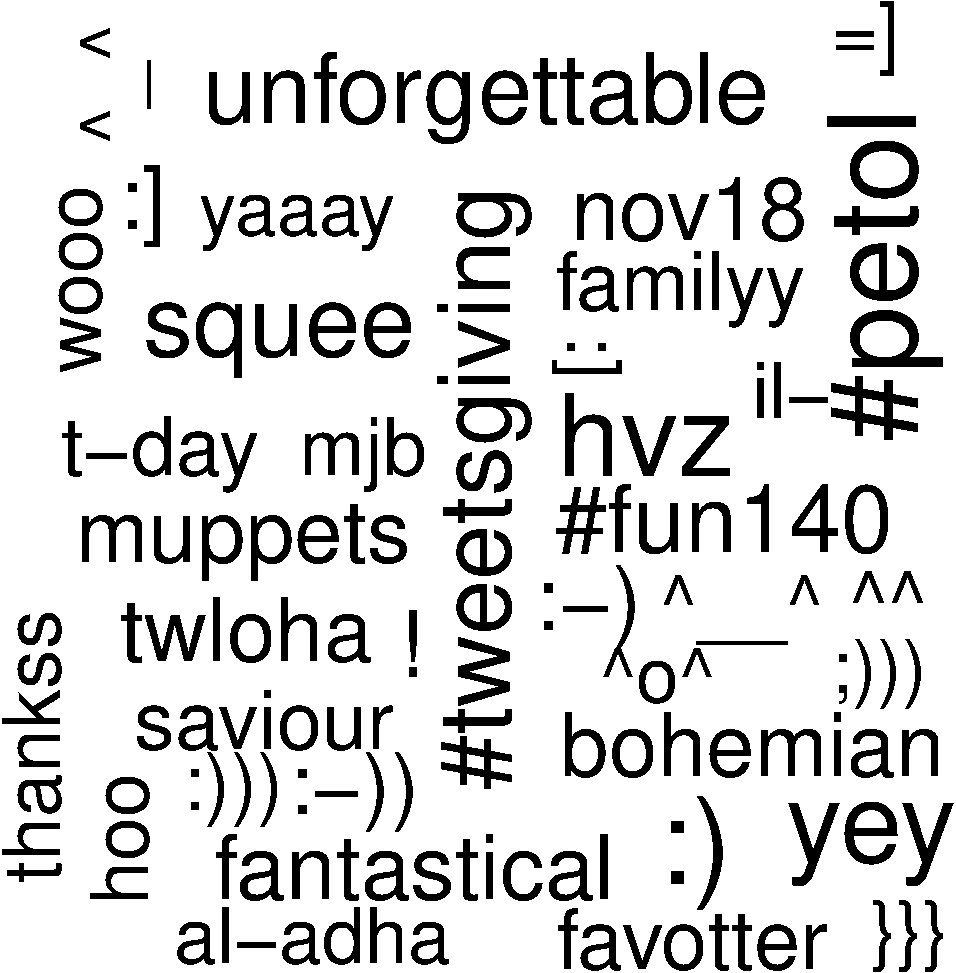
\includegraphics[scale=0.2]{pics/joy.pdf} & 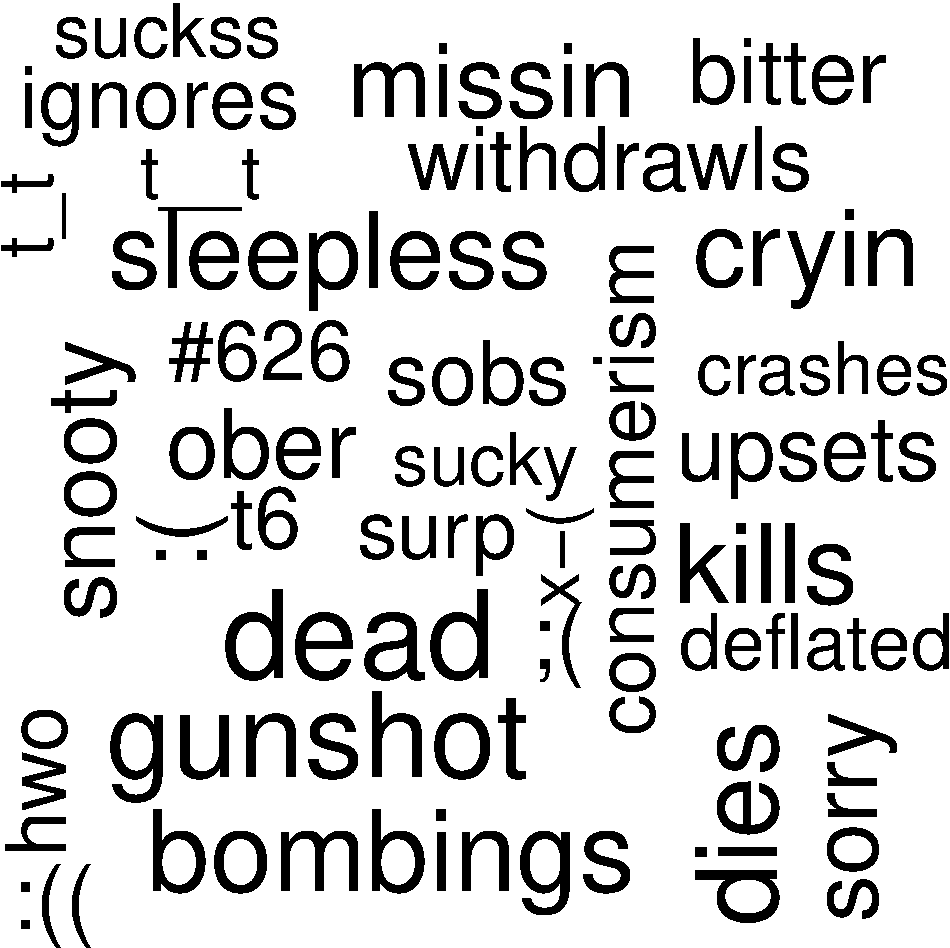
\includegraphics[scale=0.2]{pics/sadness.pdf} & 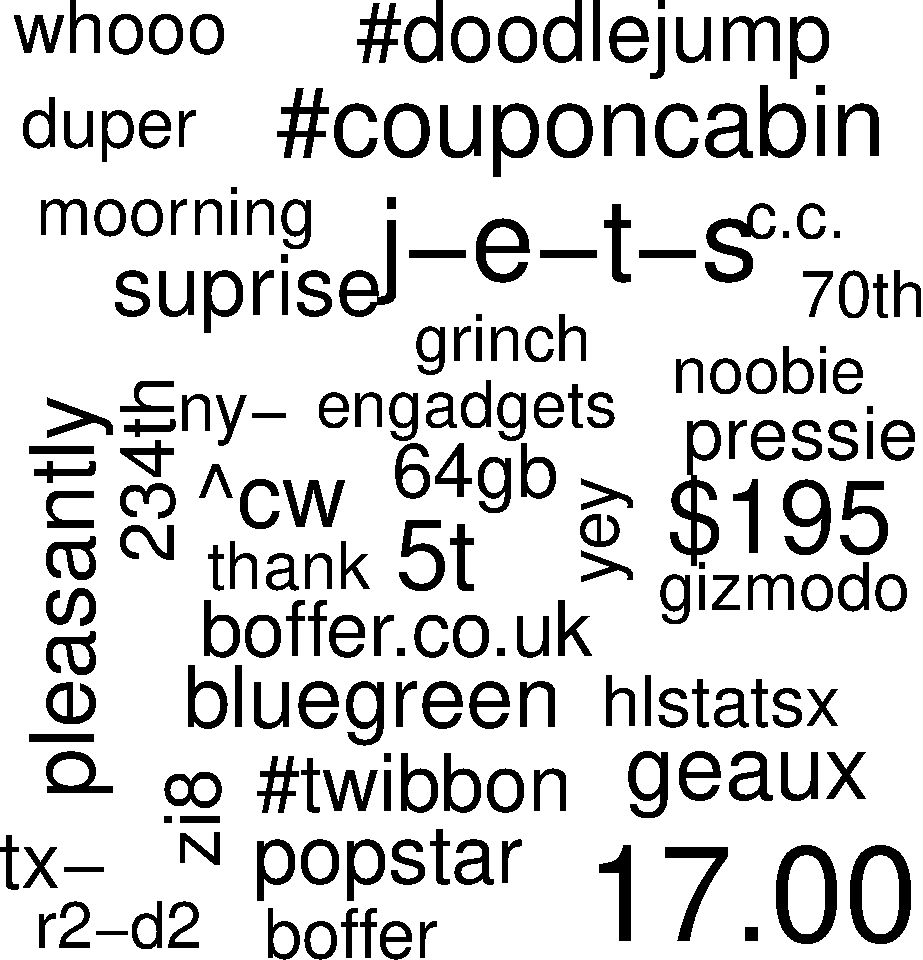
\includegraphics[scale=0.2]{pics/surprise.pdf} & 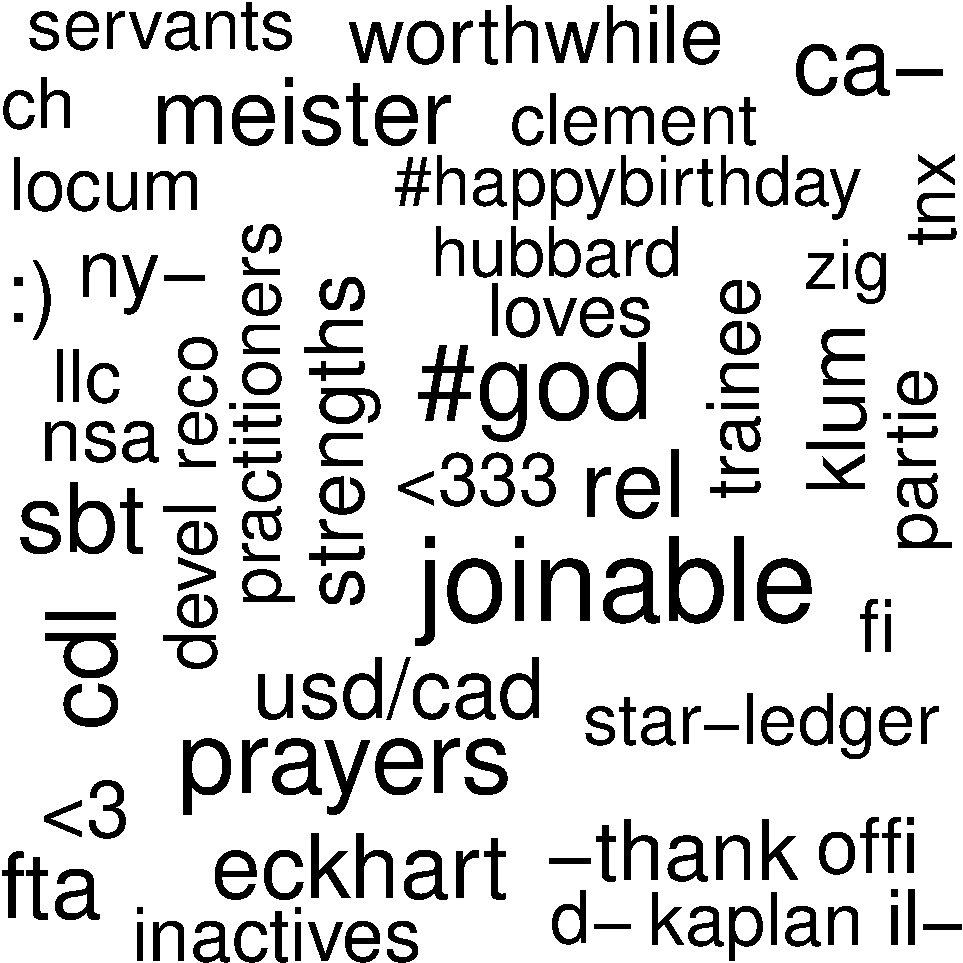
\includegraphics[scale=0.2]{pics/trust.pdf} \\
joy & sadness & surprise & trust\\
\end{tabular}}
\end{center}
\end{figure}

\end{scriptsize}
\end{frame}